\documentclass[14pt,fleqn]{extarticle}
\RequirePackage{prepwell}

\previewoff

\begin{document} 
\begin{skill}
    \begin{narrow}
         \textcolor{blue}{Ellipse Basics}
    \end{narrow}
    
    \reason 
    
    \begin{center}
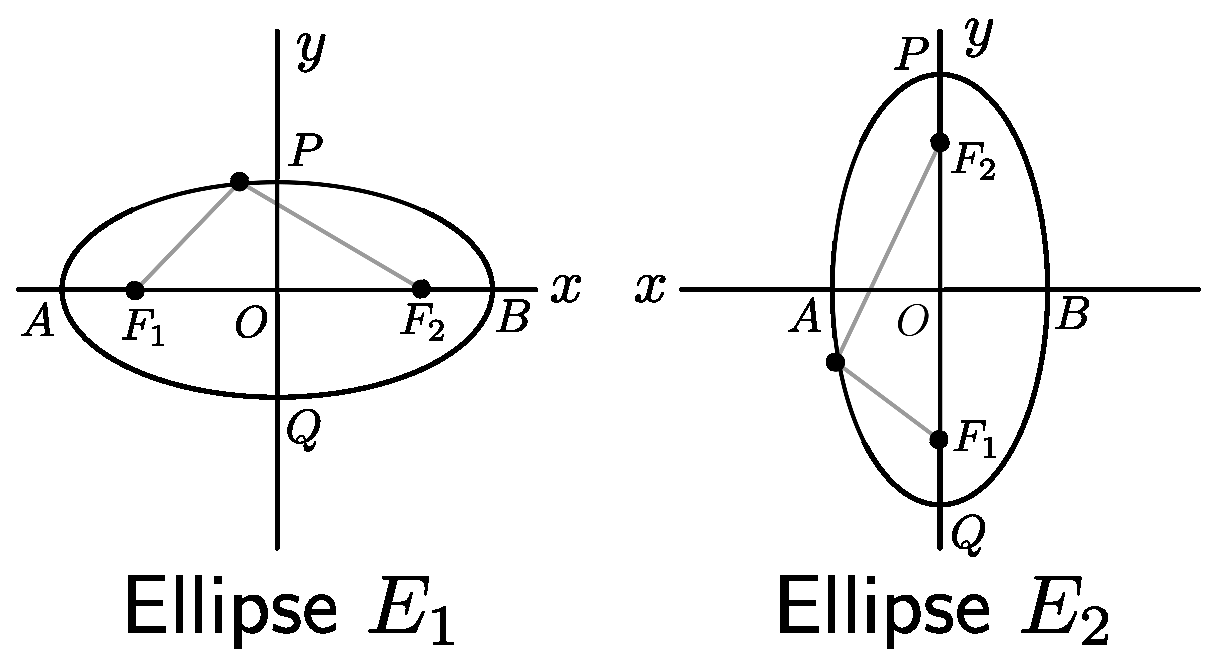
\includegraphics[scale=0.4]{figure.eps}
\end{center}

An ellipse is the locus of all points the sum of whose distances 
from two fixed points (the foci) is constant \newline 

Shown above are two ellipses. The following is common to both 

\begin{center}
  \begin{tabular}{Nl}
   \toprule
        & Meaning \\
   \midrule 
   O & The center. When $F_1,F_2$ and $O$ \\
   & coincide, then we have a circle \\ 
    \midrule 
    F_1 \text{ and } F_2 & The foci. Always on the major-axis \\
    \bottomrule
  \end{tabular}
\end{center}

And this is how they differ. Remember \underline{$a > b$ in the equations below}

\begin{center}
  \begin{tabular}{cNN}
   \toprule
        &  \text{Ellipse }E_1 & \text{Ellipse }E_2 \\
   \midrule 
   Major axis & AB & PQ \\
    \midrule 
    Minor axis & PQ & AB \\
    \midrule 
    Equation & \frac{x^2}{a^2} + \frac{y^2}{b^2} = 1 & \frac{x^2}{b^2} + \frac{y^2}{a^2} = 1 \\
    \midrule 
    Parametric & x = a\cos\theta & x = b\cos\theta \\
    & y = b\sin\theta & y = a\sin\theta \\
    \bottomrule
  \end{tabular}
\end{center}
    
\end{skill}
\end{document} 